\section{KevoreeJS: A runtime for reconfigurable single page applications in the browser}

This section present a module system for the Browser called KevoreeJS .
%\ff{Just matter of presention, but i think we not target JS, we target the brower USING javascript. But the goal is really to target a usage and not a language no ? The language is a way todo.}
In particular, KevoreeJS implements a dynamic component model for SPA.
This component model currently addresses only a part of the challenges discussed in Section 2.

\subsection{Motivating Scenarios }
To illustrate the framework, we consider a simple dashboard for sensor-based system in which, it is required to install/uninstall a new web widget when a new sensor appears/disappears. In such system, three kinds of reconfiguration have to be managed: i) the installation and retrieval of software package (javascript code), the instantiation of components, the components parametrization (to bind components through ports, the setup of parameters, ...), the component life-cycle management. ii)  the client/server code partitioning to select if some components managing complex event queries must be executed on the server side or within the browser. iii) the selection of a specific deploy unit depending on the browser type, its devices and its screen layout. A screenshot of the results of such an application is presented in Figure\ref{fig:fig1}. This dashboard provides information regarding values that can come from a set of nodes such as the one described in Figure~\ref{fig:fig2}.


\begin{figure*}[h]
	\center
	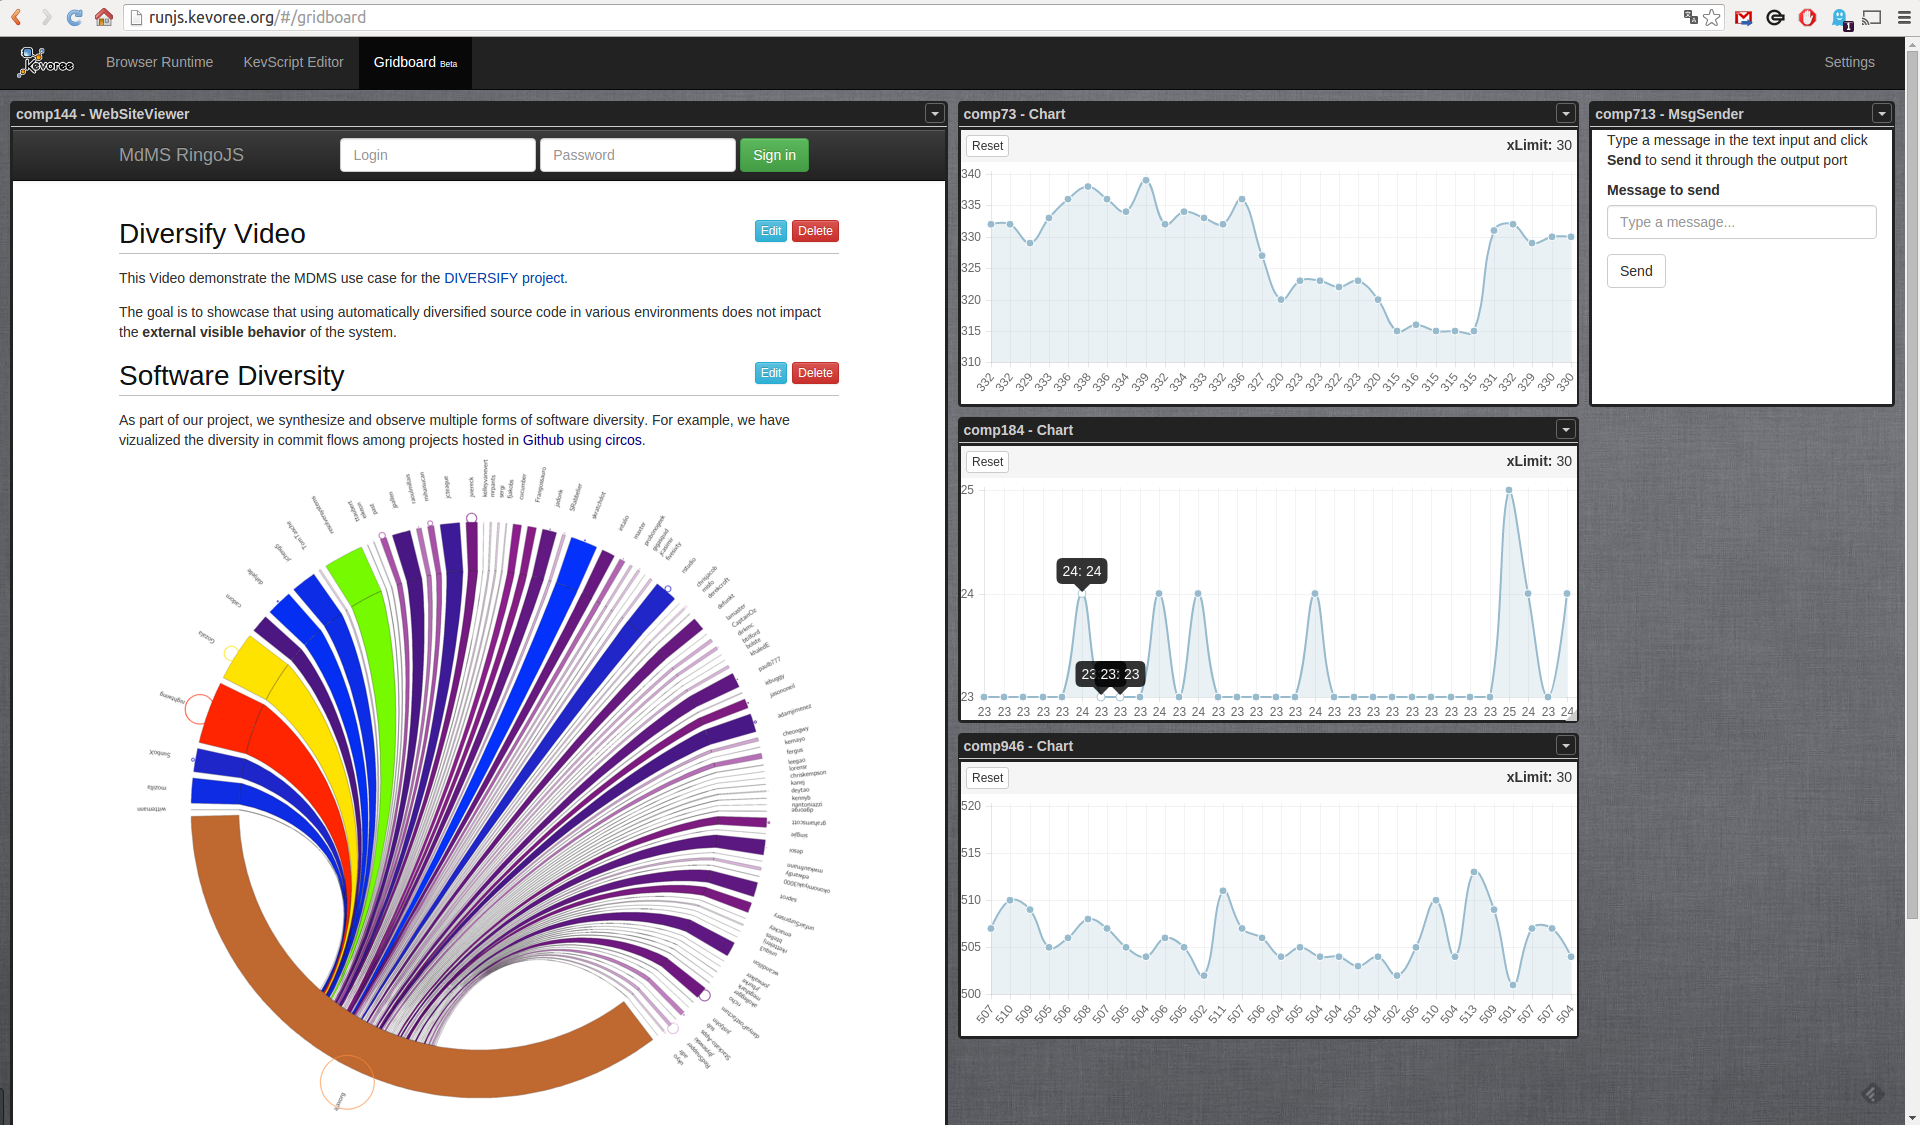
\includegraphics[width=1\textwidth]{figures/fig3}
	\caption{An example of dashboard for sensor-based applications}
	\label{fig:fig1}
\end{figure*}


\begin{figure}[h]
	\centering
	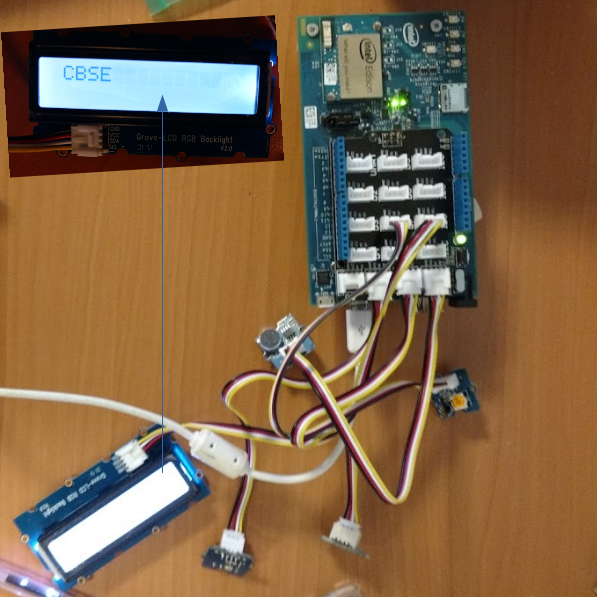
\includegraphics[width=0.8\linewidth]{figures/fig4}
	\caption{An example of sensor node based on Intel Edison}
	\label{fig:fig2}
\end{figure}


\subsection{KevoreeJS overview }
KevoreeJS is built on top of the models@runtime paradigm. Models@runtime denotes model-driven approaches aiming at taming the complexity of dynamic adaptation. It basically pushes the idea of reflection~\cite{DBLP:conf/icse/MorinBNJ09} one step further by considering the reflection layer as a real model that can be used to drive the system deployment and (re) configuration: ``something simpler, safer or cheaper than reality to avoid the complexity, danger and irreversibility of reality''. In practice, component-based (and/or service-based) platforms like Fractal~\cite{bruneton2006fractal}, OpenCOM~\cite{grace2005reflective} or OSGi~\cite{hall2011osgi} offer reflection APIs which make it possible to introspect the system (which components and bindings are currently in place in the system) and dynamic adaptation (by applying CRUD operations on these components and bindings). While some of these platforms offer rollback mechanisms~\cite{david2006safe} to recover after an erroneous adaptation, the idea of models@runtime is to prevent the system from actually enacting an erroneous adaptation. In other words, the ``model at runtime'' is a reflection model which can be uncoupled (for reasoning, validation, simulation purposes) and automatically resynchronized. This modelling layer provides a common abstraction to describe the system configuration. This model can be interpreted to decide which packages (component package and third parties libraries) must be installed or removed and which component must be instantiated and started. This modelling layer can also be  modified and pushed to peers to trigger distributed reconfigurations.

KevoreeJS\footnote{http://runjs.kevoree.org}  implements the Kevoree component model. Kevoree is a dynamic component-based framework for distributed systems that follows the models@runtime paradigm and embeds a structural model of the distributed system. This model is used for two main purposes: (i) it represents a snapshot of the heterogeneous and distributed application state and (ii) it provides a language to drive the reconfigurations of this application. The Kevoree model embodies the following four main concepts of a distributed system.

\begin{enumerate}
	\item The software \textbf{components} represent software units that provide the business value of the distributed system.
\item The \textbf{connectors} (called channels in Kevoree) are in charge of inter-component communications. A channel encapsulates and provides a particular communication semantic (e.g. synchronous or asynchronous, unicast or multicast, and may provide different contracts for synchronization and quality of services).
\item The \textbf{nodes} represent execution hosts for all other software entities such as components and channels. A node may represent a physical node or a virtual machine. Nodes are application containers and they are in charge of the dynamic adaptations of its system part when a new model@runtime is received.
\item The \textbf{groups} are responsible for inter-node communications. In particular, a group provides semantics of dissemination and ensures consistency of models among nodes. On top of these abstractions, Kevoree provides a development model to design new components, channels, groups and nodes using different programming languages. It also comes with a set of tools for building dynamic applications (a graphical editor to visualize and edit configurations, a textual language to express reconfigurations, several checkers to validate configurations). Kevoree supports multiple execution platforms (e.g., Java, JavaScript, .NET, Android, LXC, Docker, FreeBSD, Arduino). For each target platform it provides a specific runtime container as a specific node type.

\end{enumerate}


For supporting the SPA within the browser, we mainly reused the core of Kevoree component model which is written in Kotlin. This core contains the component model entities, tooling for loading and saving configuration models, tooling for detecting abstract actions (install a library, instantiate a component, bind a component to a channel, \dots)  and tooling to achieve runtime adaptations when the platform receives a new configuration model. As Kotlin provides a code generator for JavaScript, we can reuse this core library directly. As a consequence, to create KevoreeJS we mainly provide the concrete implementations of abstract actions in order to achieve concrete tasks within a running Browser core. We also provide a basic UI composition mechanism based on mashup. Each component comes with its own view that can be composed on the full SPA using mashup. To enable this mashup mechanism, we reuse framework such as AngularJS and angular-gridster. KevoreeJS reuses Bower for its static Web part, but it handles the dynamicity by downloading browserified\footnote{http://browserify.org/} modules directly from the npm registry.




Finally we provide a simple development model in JavaScript and in TypeScript for developing components, channels, groups and nodes.

KevoreeJS comes with a set of tools: a web-based architecture model editor, a Yeoman generator, a set of Grunt tasks to fully automate the component packaging and publishing and a runtime container to manage the dynamic deployment of third-party libraries.



The yeoman generator create skeletons to implement new components. It provides six Software artefacts:
\begin{itemize}
	\item package.json, which defines the set of dependencies for your component
	\item Gruntfile.js, which provides the tasks to achieve for creating your component deployment unit. 
	\item  browser/kevoree-comp-mycomp.html, as we reuse angularJS as a development model for the component, this html file is the view of your component.
	\item lib/MyComp.js,  as we reuse angularJS as a development model for the component, this JavaScript file contains the model and the controller for your component.
	\item browser/ui-config.json; this file serves to configure the style parameters, the layout parameters, the angularjs module dependencies parameter and the other JavaScript artefacts to include. 
	\item kevs/main.kevs; this file contains an initial configuration when starting the application. 
\end{itemize}


\subsection{Development model}
To illustrate this development model, we discuss the code of the last four artefacts for a component that has the following view (see Figure~\ref{fig:fig5}).


\begin{figure}[h]
	\centering
	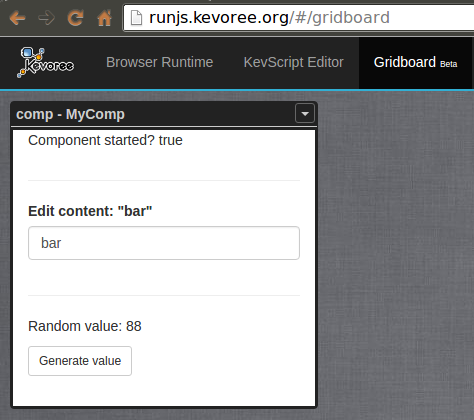
\includegraphics[width=0.8\linewidth]{figures/fig5}
	\caption{An example of KevoreeJS component}
	\label{fig:fig5}
\end{figure}

The view contains the following html code. It can access to component attribute such as the life cycle state or business value (\emph{foo} or \emph{value}). It can also act on the component internal behavior in calling specific function declared in the component implementation (\emph{genValue}).

\begin{lstlisting}[language=HTML,numbers=right,firstnumber=last]
<div class="col-xs-12">
<p>Component started? {{ started }}</p>
</div>
<div class="form-group col-xs-12">
<hr />
<label for="foo">Edit content: "{{ foo }}"</label>
<input type="text" class="form-control" id="foo" data-ng-model="foo">
</div>
<div class="col-xs-12">
<hr />
<p>Random value: {{ value }}</p>
<button class="btn btn-sm btn-default" data-ng-click="genValue()">Generate value</button>
</div>
\end{lstlisting}


The component implementation contains the following JavaScript code. Implementing a component consists in defining its life-cycle methods (start and stop, l 18-34), defining some parameters that can be configured from the configuration model (l 4-9) and defining the uiControler that will be invoked from the browser runtime to create the graphical views of the component. The binding between the views and the component model is obtained in sharing the \emph{\$scope} object  that refers to the application model in the angularJS technological stack. The developers can also define input and output ports for the component\footnote{https://github.com/kevoree/kevoree-js}). We propose an alternate development model using TypeScript as a main programming language. 



\begin{lstlisting}[language=JavaScript,numbers=left,firstnumber=1,basicstyle=\scriptsize,deletekeywords={port}]
var AbstractComponent = require('kevoree-entities').AbstractComponent;

var MyComp = AbstractComponent.extend({
 toString: 'MyComp',

/* This is an example of dictionary attribute that you can set for your entity */
dic_yourAttrName: {
	optional: false,
	defaultValue: 'aDefaultValue',
},

construct: function () {
	this.scope ={};
},

/**
* this method will be called by the Kevoree platform when your component has to start
* @param {Function} done
*/
start: function (done) {
	this.log.debug(this.toString(), 'START');
	this.scope.started= true;
	done();
	//...
},

/**
* this method will be called by the Kevoree platform when your component has to stop
* @param {Function} done
*/
stop: function (done) {
	this.log.debug(this.toString(), 'STOP');
	this.scope.started= stop;
	done();
},


/**
* this method is called by the Browser Runtime in order to retrieve
* this component AngularJS UI controller
*/
uiController: function () {
return ['$scope', '$timeout', 'instance', function ($scope, $timeout, instance) {
	// this is your UI controller function
	// $scope content is available directly within the browser/kevoree-comp-foocomp.html file
	instance.scope = $scope;
	$scope.started = instance.started;
	$scope.foo = 'bar';
	$scope.value = parseInt(Math.random()*100);
	$scope.genValue = function () {
		$scope.value = parseInt(Math.random()*100);
	};
	}];
}
});

module.exports = MyComp;
\end{lstlisting}


Finally, the development model contains a very simple configuration language for tweaking the component implementation. Developers can: 

\begin{itemize}
	\item change the style sheets (to add specific CSS style), 
	\item integrate other Angular modules (to integrate angularjs ui widget)  
	\item modify some user interface metadata such as the default layout for the component view. 
	\item integrate specific JavaScript artefact to load specific function or split its component implementation in several files. 
	\end{itemize}
 
 
This configuration can be done  using a JSON formatted configuration file: \emph{ui-config.json} such as the one presented below.
 
\begin{lstlisting}[language=JavaScript,numbers=right,firstnumber=1,basicstyle=\scriptsize,deletekeywords={port}]

{
	"scripts": [
	"my-local-script.js",
	"//cdn.scripts.foo/my-lib.js"
	],
	"styles": [
	"my-local-style.css",
	"//cdn.styles.bar/my-style.css"
	],
	"depModules": [
	"myNgModule"
	],
	"layout": {
		"width": 2,
		"height": 1
	}
}
\end{lstlisting}

Finally the last artefact contains the configuration model used to define the architecture of a distributed and heterogeneous application. A full documentation of this configuration can be found \cite{http://kevoree.org/doc/}. The following example  illustrates a configuration with two nodes: one that will start a Node.js runtime to provide a WebServer 
 and the other one will run in the Browser runtime. Figure~\ref{fig:fig6} presents a visual representation of this running configuration using the Kevoree Editor. 


\begin{lstlisting}[language=JavaScript,numbers=right,firstnumber=1,basicstyle=\scriptsize,morekeywords={add,attach,set,network}]
add node0, browser : JavascriptNode
add sync : WSGroup
// and we add your component to the Browser node so that you can test your UI
add browser.comp : cbse.MyComp

attach node0, browser sync

set sync.master = 'node0'

set browser.logLevel = 'DEBUG'
set browser.comp.yourAttrName = 'nonDefaultValue'

\end{lstlisting}

\begin{figure}[h]
	\centering
	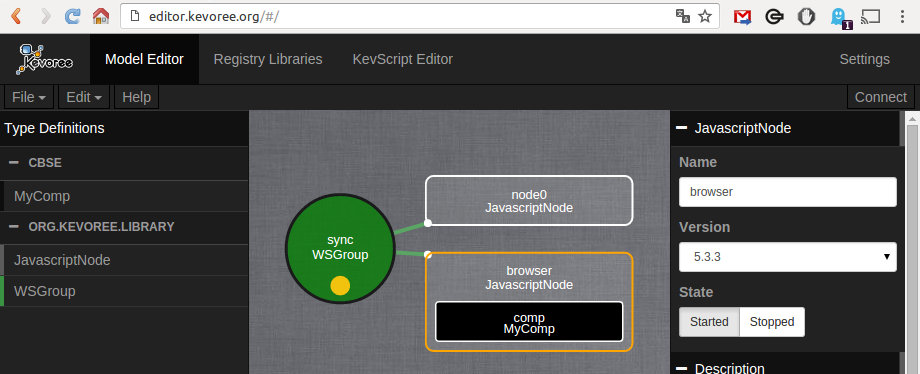
\includegraphics[width=1.\columnwidth]{figures/fig6}
	\caption{Visual editor that displays an excerpt of configuration}
	\label{fig:fig6}
\end{figure}


 A more complete description of the development model is available online\footnote{ https://github.com/HEADS-project/training/tree/master/2.Kevoree\_Basics}, \footnote{https://github.com/kevoree/kevoree-js.d.ts}.

\subsection{Evaluation}
To validate the proposed approach, we follow two ways. First we provide some figures on KevoreeJS in terms of line of code, number of reusable components available online, time penalty to initiate KevoreeJS when loading the pages. Then, we evaluate the approach regarding the challenges discussed in Section 2.

\subsubsection{Quantitative evaluation}
To implement the KevoreeJS core and the sensor based dashboard, we create 8 components, 3 channels, 3 groups. The core of KevoreeJS and these 14 software artefacts contain 56,671 LoC (15,584 has been manually written and 41,177 are generated from the model to automatically manage model entities, model load and serialization, \dots The Figure~\ref{fig:fig3}  illustrates the configuration model of the applications using the Kevoree Web Editor~\footnote{http://editor.kevoree.org}. The Figure \ref{fig:fig4} focuses in particular on the configuration of the SPA presented in Figure~\ref{fig:fig1}. All the code for this application is available on github. We provide a companion web page \footnote{http://github.com/kevoree/CBSE16KevoreeJS} to provide the links to all the software artefacts we use in this experiment.


\begin{figure*}[t]
	\centering
	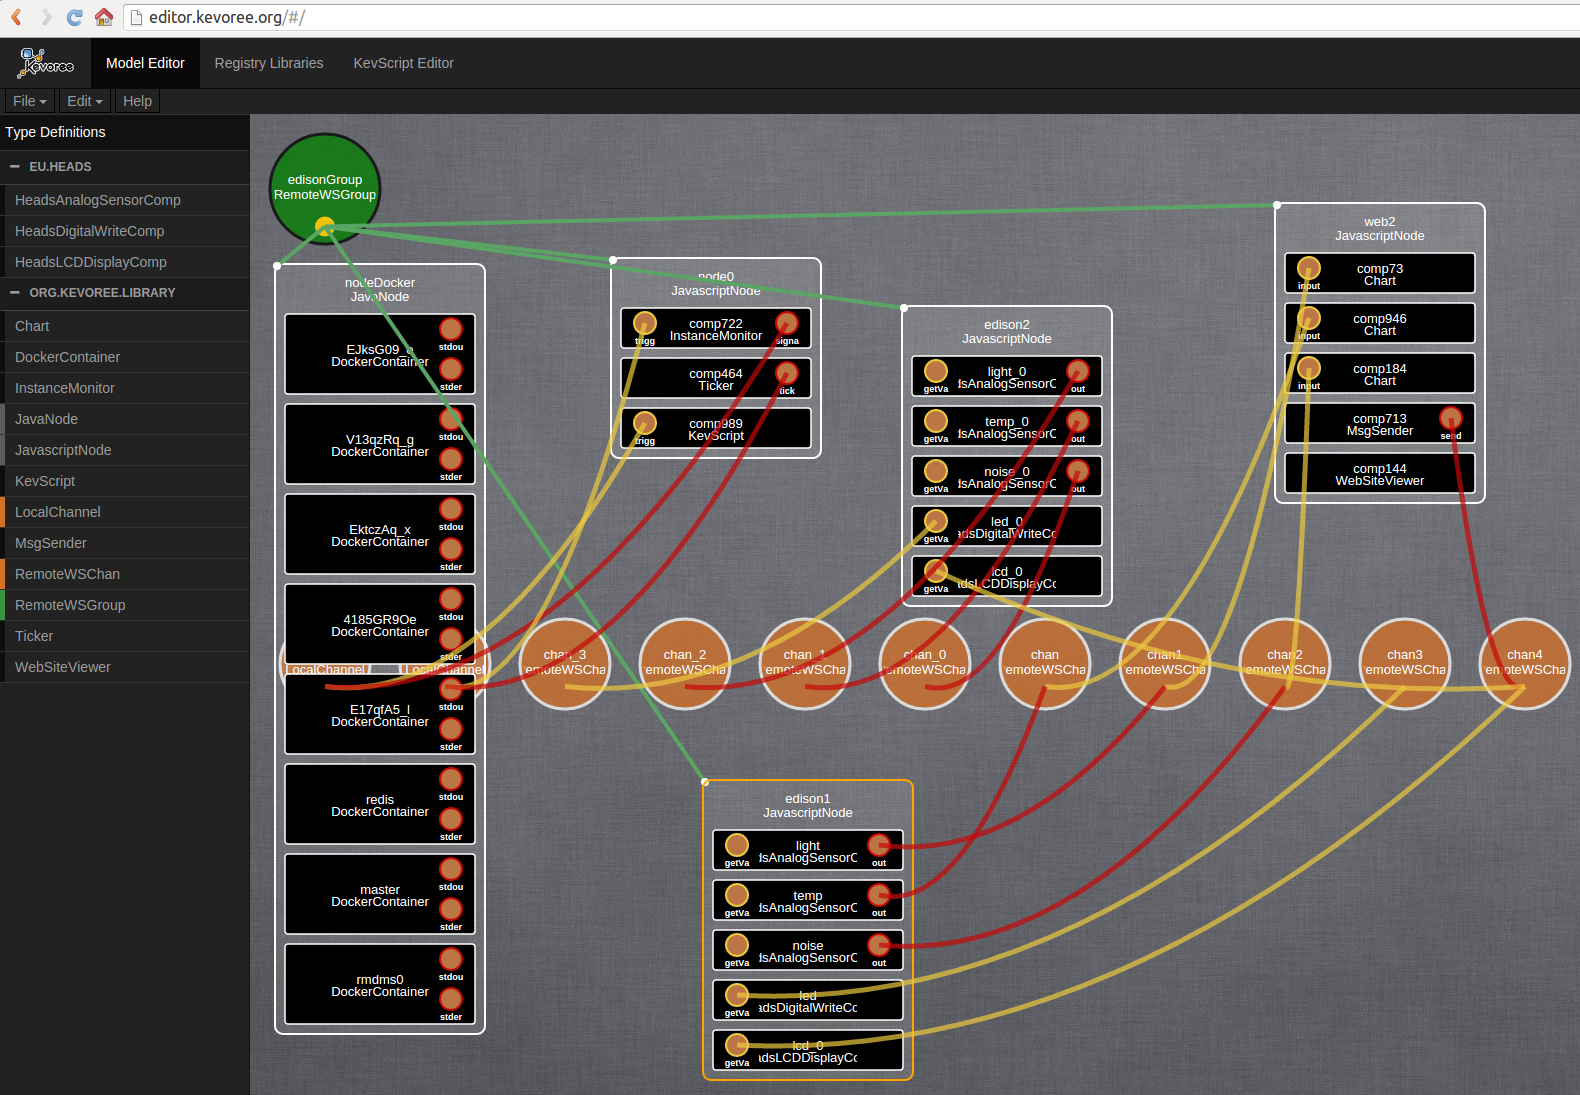
\includegraphics[width=1\linewidth]{figures/fig1}
	\caption{An example of dashboard for sensor-based applications}
	\label{fig:fig3}
\end{figure*}


\begin{figure}[t]
	\centering
	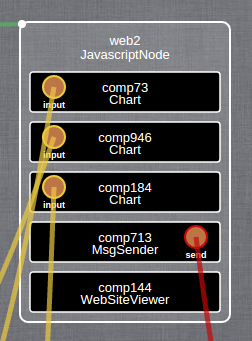
\includegraphics[width=0.5\linewidth]{figures/fig2}
	\caption{An example of sensor node based on Intel Edison}
	\label{fig:fig4}
\end{figure}


Starting the sensor based application on a Chrome browser, running on top of a HP EliteBook 820 with Intel i7 processor, SSD hard drive and 16Gbytes of memory, takes 1533 ms from scratch. It takes 677ms when the components are available in the cache. The load time is mainly the time to download software modules on the npm registry server. Deploying the sensor based dashboard consists in writing a simple configuration.

\ff{Ideally here we could have a very nice graph. Like we could make vary the scale of the problem and measure the rendering/downloading/... time. This way we could conclude a bit more strongly about the overhead of browser rendering. Another point is that the server is also not under pressure to in theory we can serve more ... not easy to quickly monitor}

\subsubsection{Qualitative evaluation  }
To discuss the strength and the limitations of KevoreeJS, we present the current implementation choices regarding the challenges discussed in Section 2.

\indent \textbf{1.} KevoreeJS provides an initial solution to automatically provision component implementations and third-party libraries. It reuses npm's registry to download the component implementations. KevoreeJS does not provide isolation between components, such as sandboxing mechanism. As a result, a faulty KevoreeJS component may impact the rest of the SPA. However, components' UIs are displayed using iframes which helps sandboxing the CSS.

\indent \textbf{2.} KevoreeJS provides a basic type system inherited from the Kevoree component to check component assembly description. The provided development environment also support TypeScript to ensure interface compatibility between components.

\indent \textbf{3.} KevoreeJS provides an initial UI composition mechanism based on mashup. If this UI composition mechanism is sufficient for a sensor based dashboard, currently KevoreeJS does not provide advanced UI composition mechanism.

\indent \textbf{4.} KevoreeJS provides an initial security solution to restrict peers access to the model configuration. This mechanism is currently limited in its ability to manage role based access rules on the configuration models. KevoreeJS relies on registries, which act as providers of the model characteristics. On this aspect, KevoreeJS has to deal with the same issues of trustability than the Linux distribution providers (e.g debian's apt, arch's linux pacman...) have encountered in the past (i.e. what happened if an attacker corrupt a registry and reference a malware?).  In its current implementation, by default, Kevoree is unsecured.

\indent \textbf{5.} Search Engine Optimization is still an open problem. We do not provide new concepts in the KevoreeJS to solve this issue.

\indent \textbf{6.} We support client/server partitioning. Among 14 modules that have been developed for the motivating scenario, 11 are cross-platform Java-JavaScript components, consequently they can run on the server side or on the client side.  One of the component, which is in charge of doing complex event processing is generated from ThingML behavioral description. ThingML~\cite{DBLP:conf/models/FleureyMSB11} provides code generators for Java, JavaScript, and C. Consequently this component can be deployed dynamically on the Browser or within a Java or JavaScript Kevoree runtime on the server.  The following code illustrates an example of a component behavior that perform a complex event processing on a stream of float value and provide every five second an average of this stream of values. Thanks to thingML code generators, we could obtain C, Java or Javascript implementation of this behavior. Consequently, an architect can dynamically decide if the query must be deployed closed to the sensors, within a gateway or within the bowser. 

\begin{lstlisting}[language=ThingML]
thing CepComp {
	message input(v : Float);
	message output(avg : Float);
	
	required port cep {
		receives input
		sends output	
	}
	
	function avg(values : Float[]) : Float do
		var i : Integer = 0
		var appen : Float = 0
		while(i < values.length) do
			appen = appen + values[i]
			i = i+1
		end
		return appen / i
	end
	
	stream computeAvg do
	from evt : [cep?input]::timeWindow(5000, 5000)
	select avg : avg(evt.v[])
	action cep!output(avg)
	end
	
	statechart behavior init Init {
		state Init {
			on entry print("Starting")			
		}
	}
	
}
\end{lstlisting}



\indent \textbf{7.} We take the design decision in KevoreeJS that the browser history only affect the component states. We do not use Browser history API to go back to a previous SPA configuration.

\indent \textbf{8.} Improving analytics in dynamically adaptable SPA is still an open problem in our current implementation of KevoreeJS

\indent \textbf{9.} Finally, the KevoreeJS core takes 20kbytes without any minification. The use of KevoreeJS does not have any real impact on the SPA performance using standard browser and hardware.
